\documentclass{article}
\usepackage[utf8]{inputenc}
\usepackage{amsmath}
\usepackage{amsfonts}
\usepackage{amssymb}
\usepackage{geometry}
\geometry{margin=1in}
\usepackage{microtype}
\usepackage{graphicx}
\usepackage{subcaption}
\usepackage{float}

\title{July 2025 Summary}
\author{Research Notes}
\date{July 2025}

\begin{document}
\maketitle

\section{July 2025 Research Summary}

\subsection{Galene-Simulator Comparison for 2D Nanowire Structures}
Comprehensive comparison between Galene and our simulator for 2D nanowire structures.

First, I expanded the current Galene code in our simulator. It is now a comprehensive Galene converter which can convert Galene simulation results (.OSV files and .GEO files) into other formats as required, such as MATLAB or for TikZ plots.

For comparison, I present the electron density and potential at a surface plot and at a slice here. The device structure we simulated is a double gate MOS structure, serving as the starting point to study the nanowire MOSFET. Here we use voltages for both gates $V_{gt}$ and $V_{gb}$ of 1.0 V and also a drain voltage $V_d$ of 1.0 V, with velocity saturation neglected (the saturation velocity in Galene is set to $10^{20}$ cm/s while velocity saturation in our simulator is turned off).

\begin{figure}[htbp]
    \centering
    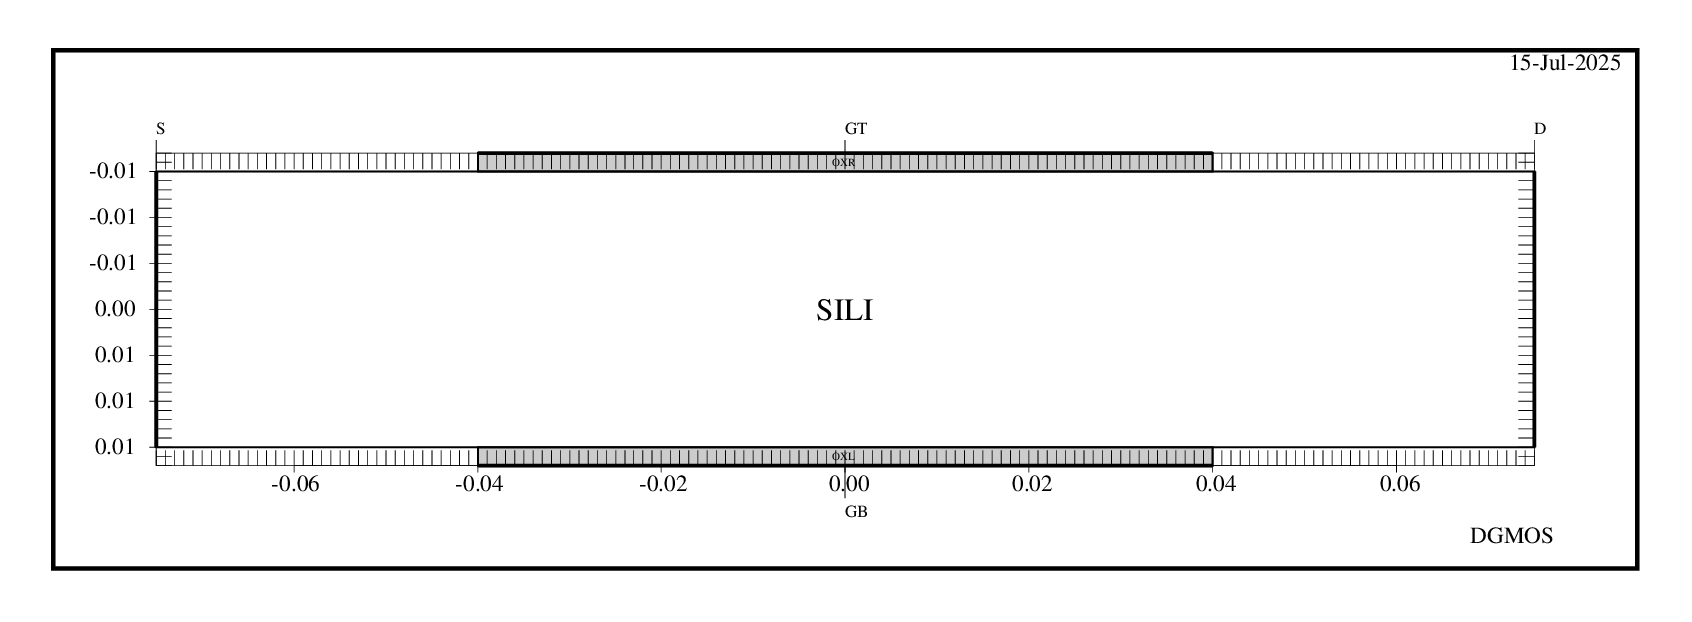
\includegraphics[width=0.8\textwidth]{Figs/dgmos.png}
    \caption{Double gate MOS device structure used as the foundation for nanowire MOSFET studies. Device parameters: length $L = 150$ nm, width = 30 nm, gate length $L_g = 80$ nm, doping regions $L_{dop} = 35$ nm, with doping concentrations $N_{d1} = 10^{20}$ cm$^{-3}$ and $N_{d2} = 10^{15}$ cm$^{-3}$. Oxide thickness $d_{ox} = 2$ nm.}
    \label{fig:dgmos}
\end{figure}

\begin{figure}[H]
    \centering
    \begin{subfigure}[b]{0.48\textwidth}
        \centering
        \includegraphics[width=\textwidth]{Figs/pot_comp.pdf}
        \caption{Potential density comparison}
        \label{fig:potential_comp}
    \end{subfigure}
    \hfill
    \begin{subfigure}[b]{0.48\textwidth}
        \centering
        \includegraphics[width=\textwidth]{Figs/ndens_comp.pdf}
        \caption{Electron density comparison}
        \label{fig:ndens_comp}
    \end{subfigure}
    \caption{Comparison between Galene and our simulator for the 2D nanowire structure. For both subfigures: the first row shows the simulation result from Galene, the second row shows the result from our simulator, the third row is the difference between the two.}
    \label{fig:comparison}
\end{figure}

From the simulation results, it can be seen that the potential and electron density are in good agreement between Galene and our simulator. For the potential difference, it is mainly due to how the simulator handles the region outside the solution domain. As for the carrier density, the deviation is mainly at the doping transition region, which is expected due to different doping mapping approaches used by both simulators.

Here, a comparison of the potential and electron density at a cross-sectional slice is shown. This represents the profile along the surface at y=0.

\begin{figure}[H]
    \centering
    \begin{subfigure}[b]{0.48\textwidth}
        \centering
        \includegraphics[width=\textwidth]{Figs/pot_x_cut.pdf}
        \caption{Potential density slice comparison}
        \label{fig:potential_slice}
    \end{subfigure}
    \hfill
    \begin{subfigure}[b]{0.48\textwidth}
        \centering
        \includegraphics[width=\textwidth]{Figs/ndens_x_cut.pdf}
        \caption{Electron density slice comparison}
        \label{fig:ndens_slice}
    \end{subfigure}
    \caption{Cross-sectional comparison between Galene and our simulator along the y=0 surface.}
    \label{fig:slice_comparison}
\end{figure}


Up to this point, the grid spacing is set to 1 nm for both simulators. Figure~\ref{fig:refined_comparison} shows that after using a refined grid (0.5 nm) in Galene, the deviation regarding the electron density is reduced.
\textbf{Note:} The doping profile mapping into Galene is still under investigation. Our simulator uses a node (vertex) centered doping mapping, while it remains to be confirmed whether Galene uses the same approach or an element-centered mapping.

\begin{figure}[H]
    \centering
    \begin{subfigure}[b]{0.48\textwidth}
        \centering
        \includegraphics[width=\textwidth]{Figs/ndens_zoom_comp.pdf}
        \caption{Electron density comparison at slice with 1 nm and 0.5 nm grid spacing}
        \label{fig:ndens_zoom}
    \end{subfigure}
    \hfill
    \begin{subfigure}[b]{0.48\textwidth}
        \centering
        \includegraphics[width=\textwidth]{Figs/ndens_comp_refined.pdf}
        \caption{Refined grid electron density comparison}
        \label{fig:ndens_refined}
    \end{subfigure}
    \caption{Grid refinement analysis showing electron density comparison. (a) Comparison at a slice with grid spacing of 1 nm and 0.5 nm. (b) Demonstrates that with a refined grid, the deviation between simulators is reduced.}
    \label{fig:refined_comparison}
\end{figure}

\subsection{Vertical FET Structure with Perforated Source}
 The current workaround is to use a partially doped active layer with ohmic contact as a substitute for the Schottky contact. This approach allows us to proceed with simulations while we work on integrating the Schottky contact feature into our simulator.

\subsection{Schottky Contact Implementation}
The current version of our simulator does not support Schottky contacts. To simulate the devices like RFET or VFET, the implementation of Schottky contact is necessary.
For the current ohmic contact, we have charge neutrality $n_0-p_0 = N_D - N_A$ and equilibrium assumed, which for Boltzmann statistics gives:
$\phi = V_k + \frac{kT}{q} asinh \left( \frac{(N_D - N_A)}{2 n^2_{i,eff}} \right)$

in the Schottky contact case,
$\phi = V_k - \phi_B + \frac{kT}{q} \ln \left( \frac{N_C}{n_{i,eff}} \right)$
is used.

Another aspect to consider is the different type of BC, instead of the Dirchlet BC, here a Robin (mixed) BC is used, which gives:
$J_n (vector) \cdot n(vector) = q v_n (n-n^B_0)$
$j_P$ Here
with
$n^B_0 = N_c exp(-qphi_B/kT)$
and $p^B_0 = N_v exp(-qphi_B/kT)$

where phi_B is the barrier height (the difference between the contact workfunction and the electron affinity of the semiconductor). v_n and v_p are the thermoionic emission velocities for electrons and holes, respectively n0B and p0B are the equilibrium densities.




\subsection{Week 3 (July 15th)}
\section{Doping Profile Mapping}


Today's work focused on understanding how the doping profile maps onto the simulation grids in both Galene and our own simulator. This mapping is crucial for accurately comparing simulation results. Currently, we are using a uniform grid spacing of 1 nm. However, to precisely analyze the doping profile's mapping, we plan to double the grid density by halving the grid spacing.

Several essential plots remain pending, notably:

\begin{enumerate}
\item A current comparison plot between Galene and our simulator.
\item A detailed comparison plot after refining the grid.
\end{enumerate}

These plots will provide deeper insights into discrepancies and alignments between both simulation approaches.

\section{About the Codes}

How it works internally:

\begin{enumerate}
  \item \textbf{Direct Binary Reading:} The \texttt{gal\_file\_init} subroutine (lines 126--197) directly reads the binary OSV file using Fortran's unformatted file access. It doesn't need conversion to ASCII first.
  \item \textbf{Block-based Structure:} The OSV file contains data blocks with a specific binary format:
    \begin{itemize}
      \item Each block has a data type indicator (integer, real, or character)
      \item Block header contains: number of data elements + size of name
      \item Block name (character string)
      \item Block data (based on type)
    \end{itemize}
  \item \textbf{Data Extraction:} The \texttt{gal\_file\_get\_block} function (lines 199--212) retrieves specific data blocks by name, similar to what \texttt{gal3\_ex} would do.
\end{enumerate}

Key differences from command-line approach:

Instead of:
\begin{itemize}
  \item \texttt{gal3 -c XXX.OSV} \hspace{1em} Convert to ASCII
  \item \texttt{gal3\_ex -extract ...} \hspace{1em} Extract values
\end{itemize}

The code does:
\begin{itemize}
  \item \texttt{call gal\_fl\%init("DD.OSV")} \hspace{1em} Direct binary read
  \item \texttt{b => gal\_fl\%get\_block("n-density")} \hspace{1em} Extract by name
  \item \texttt{values = b\%rdata} \hspace{1em} Get real data
\end{itemize}

How it processes the data:

\begin{enumerate}
  \item \textbf{Units \& Normalization:} Lines 134--168 define physical units for various quantities, and \texttt{normalization\_m} handles unit conversions automatically.
  \item \textbf{Grid Integration:} In \texttt{device\_params.f90}, the galene data is integrated into the grid structure:
    \begin{itemize}
      \item Line 178: \texttt{call this\%gal\_fl\%init(gal\_filename\%s)} --- loads the OSV file
      \item Lines 184--194: Extract material information and properties
      \item Lines 517--534: Use volume descriptions to set up the computational grid
    \end{itemize}
  \item \textbf{Data Types:} The code handles three data types (lines 17--19):
    \begin{itemize}
      \item \texttt{GALDATA\_INT = 1} (integer data)
      \item \texttt{GALDATA\_REAL = 2} (real data)
      \item \texttt{GALDATA\_CHAR = 3} (character data)
    \end{itemize}
\end{enumerate}

The m4 macros handle platform-specific details like integer sizes and ensure compatibility across different systems.

This approach eliminates the need for external preprocessing tools by implementing the OSV file reader directly in Fortran, providing seamless integration with the simulation workflow.




\subsubsection{New Research Developments}
\begin{enumerate}
    \item \textbf{Design of a full comprehensive Galene tool in simulator:} Initiated development of an integrated Galene interface within our simulation framework to streamline the workflow and eliminate external tool dependencies.

    \item \textbf{Test a vertical FET structure with perforated source:} Explored vertical FET configurations using partially doped active layer with ohmic contact as a workaround to replace Schottky contact, providing a more accessible implementation path.
\end{enumerate}

\subsection{TODO Items}
\begin{enumerate}
    \item Compare Galene simulation result and result from simulator for 2D nanowire
    \item Investigate how the doping profile is mapped into the simulator
    \item Create a Galene profile to test for VFET
    \item Add the Schottky contact to own simulator
    \item Grid refinement analysis - halving grid spacing from 1 nm to 0.5 nm
    \item Current comparison plots between Galene and our simulator
    \item Detailed analysis of doping profile mapping accuracy
\end{enumerate}

\subsection{Technical Achievements}
\begin{itemize}
    \item Successfully implemented direct OSV file reading in Fortran
    \item Eliminated need for external preprocessing tools (gal3, gal3\_ex)
    \item Established seamless integration between Galene data and simulation grid
    \item Implemented proper unit normalization for physical quantities
\end{itemize}

\subsection{Next Steps}
\begin{itemize}
    \item Complete pending comparison plots
    \item Analyze results from refined grid simulations
    \item Document discrepancies and alignment patterns between simulators
    \item Prepare formal write-up for main paper draft
\end{itemize}

\end{document}
